\documentclass{article}
\usepackage{listings}
\usepackage{xcolor}
\usepackage{graphicx} % Required for inserting images
\usepackage{amsmath}
\usepackage{tikz}
% Define colors for code highlighting
\definecolor{codegreen}{rgb}{0,0.6,0}
\definecolor{codegray}{rgb}{0.5,0.5,0.5}
\definecolor{codepurple}{rgb}{0.58,0,0.82}
\definecolor{backcolour}{rgb}{0.95,0.95,0.92}
% Define style for Python code
\lstdefinestyle{python}{
    backgroundcolor=\color{backcolour},
    commentstyle=\color{codegreen},
    keywordstyle=\color{magenta},
    numberstyle=\tiny\color{codegray},
    stringstyle=\color{codepurple},
    basicstyle=\ttfamily\small,
    breakatwhitespace=false,
    breaklines=true,
    captionpos=b,
    keepspaces=true,
    numbers=left,
    numbersep=5pt,
    showspaces=false,
    showstringspaces=false,
    showtabs=false,
    tabsize=2
}

\begin{document}

\begin{titlepage}
  \centering
  \includegraphics[width=0.4\textwidth]{iithlogo.png}\par\vspace{1cm}
  {\scshape\LARGE Indian Institute of Technology Hyderabad \par}
  \vspace{1cm}
  {\scshape\Large Biomedical Imaging\par}
  \vspace{1.5cm}
\end{titlepage}

\begin{center}
  {\scshape\LARGE ct imaging \par}
  \vspace{0.5cm}
  {\Large Abhishek Amit Raje \par}
  \vspace{0.5cm}
  {\large February 2024 \par}
\end{center}
\newpage
\section{\textit{Sinogram of a Shepp Logan Phantom}}
\begin{itemize}
    \item A sinogram is a graphical representation of the intensity values obtained from a set of projections of an object. It is the projected sum of the 1D Fourier transforms taken about the image.
    \item The sinogram is represented as a 2D plot where the x-axis corresponds to the projection angle $\theta$ and the y-axis corresponds to the radial distance $\rho$. Each point in the sinogram represents the integral of the the image .
\end{itemize}

\begin{lstlisting}[language=Python, style=python, caption={Python code for generating sinogram}]
import numpy as np
import matplotlib.pyplot as plt
from skimage.data import shepp_logan_phantom
from skimage.transform import radon

def generate_sinogram_with_theta(phantom, theta, cmap='viridis'):
    sinogram = radon(phantom, theta=theta, circle=True)
    
    plt.subplot(121)
    plt.imshow(phantom, cmap='gray')
    plt.title('Shepp-Logan Phantom')

    plt.subplot(122)
    plt.imshow(sinogram, cmap=cmap, aspect='auto', extent=[min(theta), max(theta), 0, sinogram.shape[0]])
    plt.colorbar(label='Intensity')
    plt.title('Sinogram' )

    plt.show()

# Generate Shepp-Logan phantom
phantom = shepp_logan_phantom()

# Specify the sampling angle theta (in degrees) with a sampling rate of 0.05 degrees
theta_values = np.arange(0, 180,0.05)

# Generate sinogram with specified theta values
generate_sinogram_with_theta(phantom, theta_values)

\end{lstlisting}
\begin{figure}
    \centering
    \includegraphics[width=0.8\linewidth]{Sinogram.png}
    \caption{Sinogram at a sampling rate $\theta=0.5$ degree}
    \label{fig:enter-label}
\end{figure}
\newpage

\section{\textit{Filtered Back Projection}}
\begin{itemize}
    \item Filtered back projection is a reconstruction technique to obtain the image after taking the radon transform
    \item It is used to convert the sinogram back into the 2-D image that the CT scan has taken.
    \item A filter is applied to the sinogram data to bring attention to other prominient features(frquency) in the image.
\end{itemize}
\begin{lstlisting}[language=Python, style=python, caption={Python code for generating sinogram with  Mexican Hat filter}]
import numpy as np
import matplotlib.pyplot as plt
from scipy.ndimage import convolve1d
from skimage.data import shepp_logan_phantom
from skimage.transform import radon

def generate_sinogram_with_theta(phantom, theta, cmap='viridis'):
    sinogram = radon(phantom, theta=theta, circle=True)

    # Apply Mexican Hat filter
    mexican_hat_kernel = np.array([-1, 2, -1])
    filtered_sinogram = convolve1d(sinogram, mexican_hat_kernel, axis=0, mode='constant', cval=0)

    fig, axes = plt.subplots(1, 3, figsize=(15, 5))  # 1 row, 3 columns

    axes[0].imshow(phantom, cmap='gray')
    axes[0].set_title('Shepp-Logan Phantom')

    im1 = axes[1].imshow(sinogram, cmap=cmap, aspect='auto', extent=[min(theta), max(theta), 0, sinogram.shape[0]])
    axes[1].set_title('Original Sinogram')
    plt.colorbar(im1, ax=axes[1], label='Intensity')  # Add colorbar to the first subplot

    im2 = axes[2].imshow(filtered_sinogram, cmap=cmap, aspect='auto', extent=[min(theta), max(theta), 0, filtered_sinogram.shape[0]])
    axes[2].set_title('Sinogram with Mexican Hat Filter')
    plt.colorbar(im2, ax=axes[2], label='Intensity')  # Add colorbar to the second subplot

    plt.subplots_adjust(wspace=0.5)  # Adjust the width space between subplots

    plt.show()

# Generate Shepp-Logan phantom
phantom = shepp_logan_phantom()

# Specify the sampling angle theta (in degrees) with a sampling rate of 0.05 degrees
theta_values = np.arange(0, 180, 0.05)

# Generate sinogram with specified theta values and apply Mexican Hat filter
generate_sinogram_with_theta(phantom, theta_values)
\end{lstlisting}
\newpage
\begin{figure}
    \centering
    \includegraphics[width=1.4\linewidth]{sinogram_filter.png}
    \caption{Singogram with Mexican Hat Filter}
    \label{fig:enter-label}
\end{figure}
$$\textbf{Comparing Properties}$$
\begin{itemize}
    \item As Observed the Mexican Hat filter enhances certain frequency components in the sinogram while suppressing others.
    \item The sinogram with the Mexican Hat filter is has sharper features
    \item The filtering process  reduces  noise in the sinogram, leading to a cleaner representation of the object's  characteristics
\end{itemize}
\newpage
]\section{\textit{Reconstruction of  Image  }}
\begin{lstlisting}[language=Python, style=python, caption={Reconstructing Sinogram using Inverse Radon Transform}]
import numpy as np
import matplotlib.pyplot as plt
from skimage.data import shepp_logan_phantom
from skimage.transform import radon, iradon

def generate_sinogram_with_theta(phantom, theta, cmap='viridis'):
    sinogram = radon(phantom, theta=theta, circle=True)
    plt.subplot(121)
    plt.imshow(phantom, cmap='gray')
    plt.title('Shepp-Logan Phantom')

    plt.subplot(122)
    plt.imshow(sinogram, cmap=cmap, aspect='auto', extent=[min(theta), max(theta), 0, sinogram.shape[0]])
    plt.colorbar(label='Intensity')
    plt.title('Sinogram' )

    plt.show()

    return sinogram

def reconstruct_image_from_sinogram(sinogram, theta):
    reconstructed_image = iradon(sinogram, theta=theta, circle=True)

    plt.imshow(reconstructed_image, cmap='gray')
    plt.title('Reconstructed Image')
    plt.show()

# Generate Shepp-Logan phantom
phantom = shepp_logan_phantom()

# Specify the sampling angle theta (in degrees) with a sampling rate of 0.05 degrees
theta_values = np.arange(0, 180, 5)

# Generate sinogram with specified theta values
sinogram = generate_sinogram_with_theta(phantom, theta_values)

# Reconstruct the image from the sinogram
reconstruct_image_from_sinogram(sinogram, theta_values)

\end{lstlisting}
\begin{figure}
    \centering
    \includegraphics[width=0.625\linewidth]{Reconstruction.png}
    \caption{Reconstruction with Filter}
    \label{fig:enter-label}
\end{figure}
\section{\textit{Sinogram using 360-degree projection}}
$$\textbf{ Effect of Sampling Rate on Image Reconstruction }$$
\begin{itemize}
    \item Insufficient sampling can lead to decreased image reconstruction quality
    \item When the angle of sampling is too sparse, multiple white streaks appear in the image due to lack of data in the unkown region
    \item Increasing the number of projections (higher sampling rate) will improves the resolution and characteristics of the reconstructed image. 
\end{itemize}
\begin{figure}
    \centering
    \includegraphics[width=0.625\linewidth]{360.png}
    \caption{Reconstruction at sampling angle $\theta=0.5$ degree i.e 360 projections}
    \label{fig:enter-label}
\end{figure}
\section{\textit{Reconstruction Using Central Slice Theorem}}
\begin{lstlisting}[language=Python, style=python, caption={Reconstructing Sinogram using Central Slice Theorem}]
import numpy as np
import matplotlib.pyplot as plt
from skimage.data import shepp_logan_phantom
from skimage.transform import radon, iradon

# Generate Shepp-Logan phantom
phantom = shepp_logan_phantom()

# Perform Radon transform to obtain sinogram
sinogram = radon(phantom)

# Apply Central Slice Theorem by taking the inverse Radon transform
reconstructed_image = iradon(sinogram)

# Display the results
plt.figure(figsize=(10, 4))

plt.subplot(131)
plt.imshow(phantom, cmap='gray')
plt.title('Shepp-Logan Phantom')

plt.subplot(132)
plt.imshow(sinogram, cmap='viridis', aspect='auto', extent=[0, 180, 0, sinogram.shape[0]])
plt.title('Sinogram')

plt.subplot(133)
plt.imshow(reconstructed_image, cmap='gray')
plt.title('Reconstructed Image')

plt.show()

\end{lstlisting}
\begin{itemize}
    \item the Central Slice Theorem states that the Fourier transform of a 1D projection of an object is equivalent to a central line  in the 2D Fourier transform of the object itself.
\end{itemize}
\begin{figure}
    \centering
    \includegraphics[width=\linewidth]{Screenshot from 2024-02-05 23-46-27.png}
    \caption{Reconstruction using central Slice Theorem}
    \label{fig:enter-label}
\end{figure}
\newpage
\section{\textit{Reconstruction After Filtering}}
\begin{lstlisting}[language=Python, style=python, caption={Reconstructing Sinogram After Filtering}]
import numpy as np
import matplotlib.pyplot as plt
from skimage import io, color, transform, img_as_float
from skimage.metrics import mean_squared_error

# Read the image

# Convert the image to grayscale if it is RGB
if image.ndim == 3:
    image = color.rgb2gray(image)

# Convert the image to double
image = img_as_float(image)

# Display the size of the matrix
print('Size of the image:')
print(image.shape)

# Define the filters
filters = ["ram-lak", "shepp-logan", "cosine", "hamming"]

# Initialize an array to store the mean squared errors
mse = np.zeros(len(filters))

# Loop over each filter
for i, filter_type in enumerate(filters):
    # Perform the radon transform
    sinogram = transform.radon(image, theta=np.arange(180))

    # Apply the filter
    filtered_sinogram = transform.iradon(sinogram, filter=filter_type)

    # Convert the reconstructed image to double
    filtered_sinogram = img_as_float(filtered_sinogram)

    # Compute the mean squared error
    mse[i] = mean_squared_error(image, filtered_sinogram)

    # Display the filter name and corresponding mean squared error
    print(f"{filters[i].capitalize()} Filter MSE: {mse[i]:.4f}")

    # Display the images
    plt.figure(figsize=(12, 4))
    plt.subplot(131)
    plt.imshow(image, cmap='gray')
    plt.title('Original Image')

    plt.subplot(132)
    plt.imshow(filtered_sinogram, cmap='gray')
    plt.title(f'Reconstructed Image ({filter_type.capitalize()} Filter)\nMSE: {mse[i]:.4f}')

    plt.subplot(133)
    plt.plot(np.arange(180), sinogram.mean(axis=0), label='Sinogram')
    plt.legend()
    plt.title('Sinogram')

    plt.show()

\end{lstlisting}
Mean Square Error of Filters:
\begin{itemize}
    \item Filter: Ram-Lak, Mean Squared Error: 0.0006536
\item Filter: Shepp-Logan, Mean Squared Error: 0.0006555
\item Filter: Cosine, Mean Squared Error: 0.0007248
\item Filter: Hamming, Mean Squared Error: 0.0008254
\end{itemize}
We can analyze the filtering accuracy of the filter based on the the mean square error
\newpage
\section{\textit{Limitations of projection radiography}}
\begin{itemize}
    \item Projection radiography fails to provide details about the 3 dimensional structure as it provides a 2 dimensional image based on the central slice theroem.
    \item  projection radiography provides static images and not suitable for real time imaging
    \item There are multiple possibilities of distortion of the image due to external factors like patient movement,equiment malfuction.
\end{itemize}
\newpage

\begin{center}
  {\scshape\LARGE x-ray imaging \par}
  \vspace{0.5cm}
  {\Large Abhishek Amit Raje \par}
  \vspace{0.5cm}
  {\large February 2024 \par}
\end{center}
\newpage
\setcounter{section}{0}
\section{\textit{Factor Affecting SNR}}
Signal-to-Noise Ratio (SNR) in X-ray imaging is influenced by various factors
\begin{itemize}
    \item Scatter Radiation: Scatter radiation contributes to noise in the image
    \item Detector Efficiency: The efficiency of the detector in converting X-ray photons 
    \item Patient Thickness and Density: The composition and thickness of the patient's body influence the reduction in intensity of X-rays
\end{itemize}
If the SNR doubles then dose becomes four times 
\section{\textit{Beam Hardening}}
\begin{itemize}
    \item 
Beam hardening is a phenomenon in X-ray imaging that occurs when a  X-ray beam, which consists of a range of energy levels, passes through an object or a patient. As the X-ray beam pases through different materials of varying thickness and composition
\item In this process lower-energy X-ray photons are preferentially absorbed, leading to an increase in the average energy of the remaining X-ray beam.
\end{itemize}
\section{\textit{Aliasing,bandwidth limiting,Nyquist condition}}
\begin{itemize}
    \item \textbf{Aliasing}:Aliasing occurs when a signal is under sampled, causing incomplete reconstruction of the signal waveform.
    \item \textbf{Bandwidth limiting}Bandwidth limiting restricts the range of frequencies in a signal,between the bandpass range fro avoiding interference of irrelaavnt frequencies.
    \item \textbf{Nyquist condition}The Nyquist condition sampling theorem states  that the sampling rate must be at least twice the maximum frequency in a signal to prevent aliasing. This condition is   $f_{sampling}>2f_{max}$
\end{itemize}
\section{\textit{Percentage of X-rays are transmitted through the chest}}
We know percentage of X-rays transmitted through the chest,  the exponential attenuation formula:
\begin{equation}
    I=I_oe^{-ux}
\end{equation}
where:
\begin{itemize}
    \item I is the intensity of the transmitted X-rays
     \item $I_o$ is the initial intensity of the incident X-rays
     \item $u$ is the linear attenuation coefficient
     \item x is the thickness of the material.
\end{itemize}
The linear attenuation coefficient $u$ can be calculated using the half-value layer (HVL) (
H) and the formula 
\begin{equation}
    u=\frac{ln2}{H}
\end{equation}
Calculate u for muscle and bone
\[ \mu_{\text{muscle}} = \frac{0.693}{3.5 \, \text{cm}} \approx 0.198 \, \text{cm}^{-1} \]
\[ \mu_{\text{bone}} = \frac{0.693}{1.8 \, \text{cm}} \approx 0.385 \, \text{cm}^{-1} \]
\[ I_{\text{muscle}} = I_0 \cdot e^{-\mu_{\text{muscle}} \cdot x_{\text{muscle}}} = I_0 \cdot e^{-0.198 \cdot 16} \]
\[ I_{\text{bone}} = I_0 \cdot e^{-\mu_{\text{bone}} \cdot x_{\text{bone}}} = I_0 \cdot e^{-0.385 \cdot 4} \]
\[ I_{\text{total}} = I_{\text{muscle}} \cdot I_{\text{bone}} \]
Percentage of X-Ray Transmitted
$$e^{-0.198}*e^{-0.385}=e^{-0.583}=0.558$$
\section{\textit{Difference between X-Ray Images}}
\begin{itemize}

\item Higher Effective Energy (140 keV): X-rays with higher energy penetrate tissues more effectively. This  results in lower contrast in the image because the X-rays  making it challenging to distinguish between different
\item As observed the  high energy X-Ray is completly 
\item Higher Effective Energy (140 keV): The X-rays with higher energy can penetrate the body more deeply, reaching the detector with less absorption of the X-Ray
\item Lower Effective Energy (50 keV): Lower energy X-rays are more likely to be absorbed by tissues, leading to greater absorption by tissues. 
\end{itemize}
\newpage
\section{\textit{Opinion on getting Xray imaging for heart related diseases}.}
\begin{table}[h]
  \centering
  \begin{tabular}{|p{0.45\linewidth}|p{0.45\linewidth}|}
    \hline
    \textbf{Pros} & \textbf{Cons} \\
    \hline
    \begin{itemize}
      \item Diagnostic Tool: X-ray imaging can provide valuable information about the structure of the heart.
      \item Quick and Non-Invasive: X-rays are relatively quick and non-invasive compared to some other imaging modalities.
      \item Widely Available: X-ray facilities are widely available, making it a convenient option for initial screening.
    \end{itemize}
    &
    \begin{itemize}
      \item Radiation Exposure: X-rays involve exposure to ionizing radiation, which carries potential risks.
      \item Limited Soft Tissue Detail: X-rays are better at visualizing bones and dense structures but have limitations in capturing detailed images of soft tissues.
      \item May Require Contrast Agents: In some cases, contrast agents may be used, and individuals may have allergies or adverse reactions to these agents.
    \end{itemize} \\
    \hline
  \end{tabular}
\end{table}
\newpage
\section{\textit{Issue with X-Ray Machine}}
The diagram incorrectly labeled the Multitap AC transformer as a "Multiple AC transformer" and the Timing circuit as a "Counting circuit."

The operation of an X-ray machine involves various components:
\begin{itemize}
\item Multitap AC transformer: This component adjusts for incoming line variations by selecting different taps to compensate. The number of outputs, or taps, can range from 2 to many, allowing for the selection of a higher or lower voltage tap based on the required X-ray exposure intensity.

\item X-ray tube filament transformer: This transformer converts the AC line to supply power for heating the cathode filament. By selecting different taps, the filament heat can be adjusted, subsequently altering the X-ray tube current and total energy delivered to the patient.

\item X-ray tube high voltage transformer and bridge rectifier: This unit transforms the AC line into high DC voltage, essential for accelerating electrons from the cathode to the anode. The high DC voltage can be chosen using taps.

\item Timing circuit: Contrary to the mislabeling as a "Counting circuit," the Timing circuit controls the timing aspects of X-ray exposure. It includes an electronic counter that regulates the turn-on, turn-off, and duration of X-ray exposure to the patient.
\end{itemize}
\newpage
\section{\textit{Fourier Transforms and Spectra}}

\subsection*{a. $ \cos^2(k_0 z) $}

\[
\mathcal{F}\{\cos^2(k_0 z)\} = \frac{1}{2} \left[ \delta(\omega - k_0) + \delta(\omega + k_0) \right]
\]

\begin{figure}[h]
  \centering
  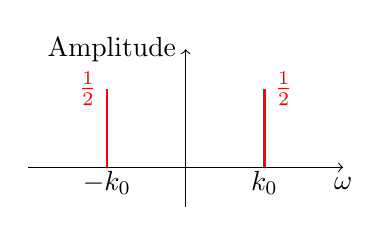
\begin{tikzpicture}
    \draw[->] (-2,0) -- (2,0) node[below] {$\omega$};
    \draw[->] (0,-0.5) -- (0,1.5) node[left] {Amplitude};

    \draw[red, thick] (1,0) -- (1,1) node[right] {$\frac{1}{2}$};
    \draw[red, thick] (-1,0) -- (-1,1) node[left] {$\frac{1}{2}$};

    \node at (1, -0.2) {$k_0$};
    \node at (-1, -0.2) {$-k_0$};
  \end{tikzpicture}
\end{figure}
\subsection*{b. $ \sin^3(k_0 z) $}

\[
\mathcal{F}\{\sin^3(k_0 z)\} = \frac{3}{4i} \left[ \delta(\omega - 3k_0) - \delta(\omega - k_0) \right]
\]

\begin{figure}[h]
  \centering
  \begin{tikzpicture}
    \draw[->] (-4,0) -- (4,0) node[below] {$\omega$};
    \draw[->] (0,-1) -- (0,1) node[left] {Amplitude};

    \draw[blue, thick] (3,0) -- (3,0.75) node[right] {$\frac{3}{4i}$};
    \draw[blue, thick] (1,0) -- (1,-0.75) node[right] {$-\frac{3}{4i}$};

    \node at (3, -0.2) {$3k_0$};
    \node at (1, -0.2) {$k_0$};
  \end{tikzpicture}
\end{figure}
\end{document}

